\documentclass[../../../../main.tex]{subfiles}
\begin{document}

\begin{flushright}
\footnotesize\textit{【自動文字起こし・要確認】}
\end{flushright}

［解］

\begin{center}
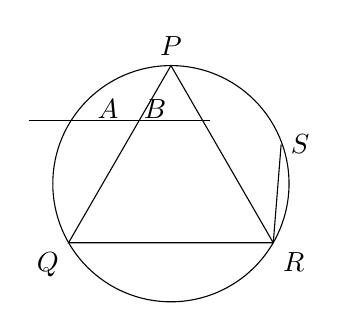
\begin{tikzpicture}[scale=1.0]
  \draw (0,0) circle (1.5);
  \coordinate (P) at (0,1.5);
  \coordinate (Q) at (-1.3,-0.75);
  \coordinate (R) at (1.3,-0.75);
  \coordinate (S) at (1.4,0.5);
  \draw (P) node[above] {$P$} -- (Q) node[below left] {$Q$} -- (R) node[below right] {$R$} -- cycle;
  \draw (S) node[right] {$S$} -- (R);
  \draw (-1.8, 0.8) -- (0.5, 0.8);
  \node at (-0.8, 0.95) {$A$};
  \node at (-0.2, 0.95) {$B$};
\end{tikzpicture}
\end{center}

$SR$ と $AB$ の交点を $C$ とおく。$P$ の位置によって，以下の2通りの位置関係がありうる。

だから，直線 $SR$ は $P$ の位置によらず，定点 $C$ を通る図。

\begin{center}
\begin{tikzpicture}[scale=0.9]
  \draw (0,0) circle (1.5);
  \coordinate (P) at (-0.4,1.45);
  \coordinate (A) at (-1.3,0.75);
  \coordinate (B) at (-0.2,0.75);
  \coordinate (C) at (0.8,0.75);
  \coordinate (Q) at (-1.4,-0.5);
  \coordinate (S) at (-0.3,-1.46);
  \coordinate (R) at (1.2,-0.9);
  \draw (-1.8,0.75) -- (1.8,0.75);
  \draw (P) node[above] {$P$};
  \draw (A) node[above left] {$A$};
  \draw (B) node[above right] {$B$};
  \draw (C) node[above] {$C$};
  \draw (Q) node[below left] {$Q$};
  \draw (S) node[below] {$S$};
  \draw (R) node[below right] {$R$};
  \draw (P) -- (A) -- (S);
  \draw (P) -- (R);
  \draw (Q) -- (S);
  \draw (S) -- (R) -- (C);
  \node at (0,-1.9) {$1^\circ$ 線分 $QS$ と $PR$ が交わらない};
\end{tikzpicture}
\qquad
\begin{tikzpicture}[scale=0.9]
  \draw (0,0) circle (1.5);
  \coordinate (P) at (0,1.5);
  \coordinate (A) at (-1.2,0.9);
  \coordinate (B) at (-0.4,0.9);
  \coordinate (C) at (1.2,0.9);
  \coordinate (Q) at (-1.45,-0.3);
  \coordinate (S) at (1.4,-0.5);
  \coordinate (R) at (0.5,-1.4);
  \draw (-1.8,0.9) -- (1.8,0.9);
  \draw (P) node[above] {$P$};
  \draw (A) node[above left] {$A$};
  \draw (B) node[above right] {$B$};
  \draw (C) node[above] {$C$};
  \draw (Q) node[left] {$Q$};
  \draw (S) node[right] {$S$};
  \draw (R) node[below right] {$R$};
  \draw (P) -- (R);
  \draw (Q) -- (S);
  \draw (S) -- (R) -- (C);
  \node at (0,-1.9) {$2^\circ$ 線分 $QS$ と $PR$ が交わる};
\end{tikzpicture}
\end{center}

$1^\circ$ の時，$PR$ と $QS$ の交点を $D$ とすると，内接四角形の対角の和が $\pi$ であることから角度が図のようになり（$\because AB \mathbin{/\!/} QS$），
\[
\triangle PAB \sim \triangle CRB
\]

$2^\circ$ の時，同じく $D$ ととると円周角の定理から $\angle QPR = \angle QSR$ であることから角度が図のようになり（$\because AB \mathbin{/\!/} QS$），
\[
\triangle PAB \sim \triangle CRB
\]

以上 $1^\circ, 2^\circ$ から，いずれの場合も $\triangle PAB \sim \triangle CRB$ であり，
$PB = x, BR = y$ とおくと
\[
BC = \frac{xy}{AB} \quad \dots \text{①}
\]
である。

\begin{center}
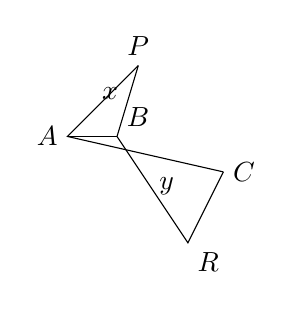
\begin{tikzpicture}[scale=0.9]
  \coordinate (P) at (0,1.5);
  \coordinate (A) at (-1,0.5);
  \coordinate (B) at (-0.3,0.5);
  \coordinate (C) at (1.2,0);
  \coordinate (R) at (0.7,-1);
  \draw (P) node[above] {$P$} -- (A) node[left] {$A$} -- (C) node[right] {$C$};
  \draw (P) -- (B) node[above right] {$B$} -- (R) node[below right] {$R$} -- (C);
  \draw (A) -- (B);
  \node at (-0.4, 1.1) {$x$};
  \node at (0.4, -0.2) {$y$};
\end{tikzpicture}
\end{center}

一方，直線 $BC$ と円の交点を $E, F$ として方べきの定理から
\[
x \cdot y = BF \cdot BE \quad \dots \text{②}
\]
①, ②から
\[
BC = \frac{BF \cdot BE}{AB} = \text{const} \quad (P \text{ の位置によらない})
\]

\newpage

\end{document}
